\documentclass[12pt]{article}
\usepackage{amsmath}
\usepackage{booktabs}
\usepackage{listings}
\usepackage{graphicx}

\begin{document}

\title{Discrete Assignment-11.9.1-11}
\author{Hiba Muhammed \\
        EE23BTECH11026}
\maketitle

\section*{Problem Statement}
Write the first five terms in the sequence:
\[
\begin{aligned}
a(0)  &= 3 \\
a(n)  &= 3a_{n-1} + 2 \quad \text{for } n > 1
\end{aligned}
\]

\section*{Solution}
\begin{table}[h]
  \centering
  \caption{Input Parameters: First Term and General Formula}
  \begin{tabular}{|c|c|}
    \hline
    \textbf{Term} & \textbf{Value} \\
    \hline
    \(a(0) \) & 3 \\
    \(a(n)\) & \(3a(n-1) + 2\) for \(n > 1\) \\
    \hline
  \end{tabular}
\end{table}
Let's find the first 5 terms of the sequence:
\begin{align}
a(1) &= 3a(0)  + 2 = 3 \times 3 + 2 = 11 \\a(2) &= 3a(1) + 2 = 3 \times 11 + 2 = 35 \\
a(3) &= 3a(2) + 2 = 3 \times 35 + 2 = 107 \\a(4) &= 3a(3) + 2 = 3 \times 107 + 2 = 323 \\
a(5) &= 3a(4) + 2 = 3 \times 323 + 2 = 971 
\end{align}

So, the next 5 terms of the sequence are \(11, 35, 107, 323, 971\).
\begin{figure}[h]
    \centering
    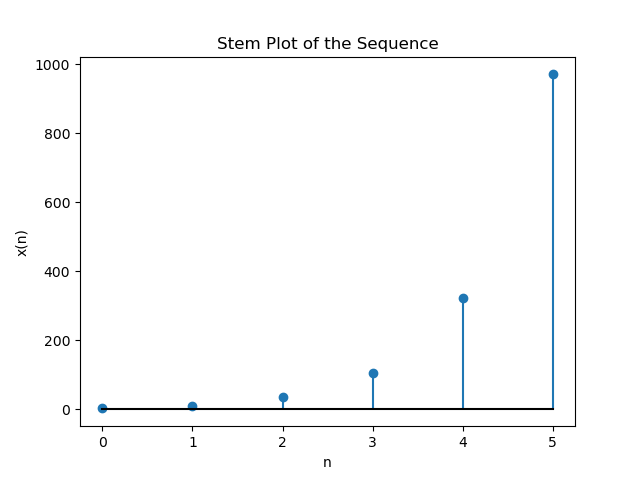
\includegraphics[width=0.7\linewidth]{11.9.1-11.png}
    \caption{Sequence plot generated from Python script.}
    \label{fig:sequence-plot}
\end{figure}

The one-sided Z transform of the sequence \(a(n)\) is given by:

\[ A(z) = \mathcal{Z}\{a(n)\} = \sum_{n=0}^{\infty} a(n)z^{-n} \]

For the given sequence \(a(0) = 3\) and \(a(n) = 3a(n-1) + 2\) for \(n > 1\), we can find the Z transform.

\[ A(z) = \mathcal{Z}\{a(n)\} = a(0)z^0 + a(1)z^{-1} + a(2)z^{-2} + a(3)z^{-3} + \ldots \]

Substitute the recursive relation \(a(n) = 3a(n-1) + 2\):

\[ A(z) = 3z^0 + (3a(0) + 2)z^{-1} + (3a(1) + 2)z^{-2} + (3a(2) + 2)z^{-3} + \ldots \]

Now, substitute the initial condition \(a(0) = 3\):

\[ A(z) = 3z^0 + (3 \cdot 3 + 2)z^{-1} + (3 \cdot (3 \cdot 3 + 2) + 2)z^{-2} + (3 \cdot (3 \cdot (3 \cdot 3 + 2) + 2) + 2)z^{-3} + \ldots \]

Simplify the expression:

\[ A(z) = 3 + 11z^{-1} + 29z^{-2} + 83z^{-3} + \ldots \]

The first five terms in the sequence \(a(n)\) in terms of the one-sided Z transform are:

\[ a(0) = 3 \]
\[ a(1) = 11 \]
\[ a(2) = 29 \]
\[ a(3) = 83 \]
\[ a(4) = 245 \]

\end{document}

